\documentclass[a4paper, titlepage]{article}

\usepackage[utf8]{inputenc}
\usepackage{hyperref} % Hyperlinks, hyperlinks everywhere
\usepackage{graphicx} % Pics or it didn't happen...

\begin{document}
	\begin{titlepage}
		\thispagestyle{empty}
		{\centering
			
\includegraphics[width=0.5\textwidth]{heriot-watt-logo.png}\par\vspace{1cm}
			%	{\scshape\LARGE Heriot-Watt University \par}
			\vspace{1cm}
			{\LARGE F28HS - Hardware Software Interface\par}
			{\LARGE Coursework 2 - ARM Assembly\par}
			\vspace{1.5cm}
			%	{\scshape\Large Coursework\par}
			\vspace{1.5cm}
			{\scshape\LARGE\bfseries Mastermind - A game of cunning and logic on the Raspberry Pi 2 \par}
			\vspace{5cm}
			
			\textit{Authors}\par
			\begin{tabular}{rcl}
				\\ \textsc{Craig James Duffy} & - & H00235298\\
				\textsc{Tommy Ian Lamb} & - & H00217505 \\
			\end{tabular} \\		
		}
	\end{titlepage}
	\pagebreak
	
	\setcounter{tocdepth}{1}
	\tableofcontents

	\clearpage
	
	
\section{Problem Specification}

The problem specification demanded an implementation of the board game Mastermind to run on the Raspberry Pi 2 using peripheral devices for user input and output. More specifically the implementation was to use two LEDs (red and green) and an LCD screen for output, and a single button for input. As a further constraint the main interaction between the software and the hardware was to be done through inline assembly. This only applied to the fundamental actions of reading and setting the state of a given pin, as well as the act of setting a pin to input or output mode. 

For the implementation of the game itself, the requirements stated that a code length of 3 should be used with 3 possible values for each position (giving $3^2 = 9$ possible permutations). 

\section{Hardware Specification}

The hardware platform for implementing the game used a single button, two LEDs (one green and one red), and a single LCD display all connected to the General Purpose Input/Out (GPIO) pins of the Pi via a breadboard. Specific details are described below.

\subsection{LEDs}

Each LED was naturally powered by a given GPIO pin, rather than getting its power from the constant 3.3V supply used elsewhere. Thus to activate or deactivate an LED, the state of given pin just needed to be set. Each LED was of course wired in series with an appropriately sized resistor to control the current flowing through the LED.
\\
\\
The red LED was connected to BCM pin 5.\\
The green LED was connected to BCM pin 6.

\subsection{Button}

The button was connected, like the LEDs, in series with a resistor to control current. However unlike the LEDs the switch was directly connected to the 3.3V supply, with a data cable connected to the circuit between the button and the downstream resistor. As such, when the button is pressed the circuit is completed and a current is allowed to flow, which produces a voltage across the data cable and its connected GPIO pin. This voltage is read as a "high" state, which is registered and acted upon by the program.
\\
\\
The data cable for the button was connected to BCM pin 19.

\subsection{LCD} 

The LCD in this implementation used the Hitachi HD44780U dot matrix LCD controller, with A00 ROM code (Japanese Standard Font) and a 40-output extension driver, giving a 16 character $\times$ 2 row display. This was connected with a data length of 4-bits due to the limited availability of cables. The LCD took two 3.3V power lines, with a potentiometer used to control the contrast on the screen. 
\\
\\
LCD pins 2 and 15 were connected to 3.3V power supply, with LCD pins 1 and 16 grounded.\\
The potentiometer also used 3.3V, with it connected to LCD pin 3.\\
LCD pin 4 (Register Select) was connected to BCM pin 25\\
LCD pin 5 (Read/Write) was connected to ground, for a permanent 0 state.\\
LCD pin 6 (Strobe pin) was connected to GPIO pin 24 \\
LCD data pins 4, 5, 6, and 7 were connected to GPIO pins 23, 17, 27, and 22 respectively.\\

\section{Code structure}

The code was dived amongst 4 separate source files: Logic, MastermindIO, GeneralIO, and LCDIO. Each is discussed separately below. 
\\
\\
To ensure proper dependency representation, both MastermindIO and LCDIO include GeneralIO with the \texttt{\#include} directive. To prevent issues with including the same file multiple times both for this project and in future, all files (except Logic.c) have inclusion guards so they are only included once when compiling. This is required as the MastermindIO file also includes LCDIO alongside GeneralIO (so GeneralIO would be included twice at compilation). The only file included in Logic.c is MastermindIO, for reasons clear below.

\subsection{Logic}

This as the name suggests is the implementation of the logic of Mastermind, and contains the main function for the software as a whole. It acts at a high level of abstraction, dealing only with the production of code sequences and processing of guesses, producing the correct values for output. No hardware details whatsoever are implemented here, rather this code makes calls to functions in the MastermindIO source file for all I/O requirements.

\subsection{MastermindIO}

MastermndIO is the source file responsible for implementation specific details, designed specifically to accommodate the requirements of the Logic file. As such, this file is where the specific pin numbers relating to LEDs, the LCD, and the button are stored as well as the memory mapped GPIO registers which get passed off to GeneralIO and LCDIO as required. This file makes calls to both the high level functions of LCDIO and the low level functions of GeneralIO in order to achieve the desired effects. While much of its work with the LCD is done through higher-level functions, for some of the special effects of the intro sequence it relies on lower-level LCDIO functions, introducing a certain amount of coupling. As part of dealing with the I/O functionality, this file also implements the multi-threading required for the input prompt on the LCD.

\subsection{LCDIO}

In order to interface easily with the LCD, this collection of functions was put together to abstract over most of the details of data transfer. It does this by implementing functions at multiple abstraction levels, each building on those below it to finally reach a high level of abstraction. As part of this abstraction, LCDIO is implementation agnostic. Of course it will only run on the Hitachi HD44780U, however it doesn't care about the specific wiring of GPIO pins, and even though it takes the memory mapped GPIO registers as an argument for most functions, it never uses them itself. Both the GPIO registers and BCM pin numbers are just passed on to GeneralIO for use in setting the appropriate pins to the appropriate values. It would have been easy to implement functions specific to the Mastermind application, however maintaining abstraction reduces coupling, making  ongoing development significantly easier, as well as producing code that may be reused in multiple different ways for various projects. 

\subsection{GeneralIO}

The bedrock of all the I/O functionality, GeneralIO represents only the lowest level, most basic functions required for any I/O operations. It specifies the inline assembly code dealing with setting the state and mode of individual GPIO pins, as well as reading in button presses and memory mapping the GPIO registers. Directly or indirectly, all of the functions declared in LCDIO and MastermindIO depend on this source file. Despite this, there is a minimal amount of coupling between the files due to the self contained nature of the functions in GeneralIO.
\pagebreak
\section{Hardware Functions}

\subsection{pinMode}

The \texttt{PinMode} function as the name suggests is used for setting the function of a pin using the GPFSEL register using a combination of C and inline assembly. C code is used for calculating the register and bit offset to simplify matters, though it should prove trivial to move the calculations into the inline assembly component. The assembly componenet takes the results alongside the address of GPIO as mapped and the function code and performs the act of writing into the appropriate GPFSEL register to set the pin mode. Before writing, the assembly zeroes the three bits in order to reset the pin function and ensure the correct 3 bits are written.

\subsection{digitalWrite}

Utilising only inline assembly, \texttt{digitalWrite} sets a given pin to either a high or low state using potentially an unintuitive methodology. In order to minimise instructions the function incrementally increases the base address of GPIO to point to the necessary register. First the address is incremented to point at GPSET0, the first of the set and clear registers. The state to set the pin to is then evaluated, with the address increased to point at GPCLR0 if the state \textbf{does not} equal 1 (so any value passed other than 1 is considered a low state). Finally the pin number itself is evaluated. If the pin is greater than 32, then the address is incremented by 4 bytes to point to either GPSET1 or GPCLR1 and 32 subtracted from the pin to give the bit offset. A single bit is written to the position indicated by the calculated bit offset in whichever register the address currently indicates.
\\ \\
As a point of further improvement, the branch instructions used can be incorporated into the instructions which they jump over. So instead of a branch condition followed by another operation which it may or may not skip, the other skipped operation can be made to execute only if the condition is met. This is possible due to the ARM assembly language, which allows certain instructions like MOV to be made conditional.


\subsection{readPin}
The pinRead function makes use of a blend of C and in-line assembly code. Using C a few variables are set-up to hold the offset  value, the value of the pin which we wish to write to in the assembly, and variable r which will ultimately decide the return value of the function. Then, the assembly makes use of the parameter pin to return its value as variable \textit{r} if \textit{r} is not equal to zero then one is returned otherwise, zero is returned. 


\section{Debug Execution}
\begin{center}
	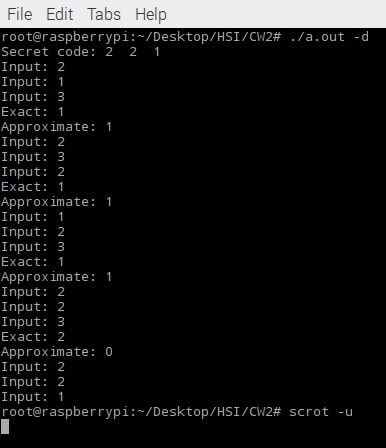
\includegraphics{Debug}
\end{center}


\section{Summary}
This project has achieved everything that it set out to achieve, with certain aspects of an especially high standard. These outstanding features include the ability to change the code length and number of colours through command arguments, the introductory sequence played out on the LCD, and the threading for LCD input prompt. In completing the coursework we have learned a great deal about low-level programming, particularly the reading of technical documentation and the application of that knowledge. Further to that we experienced programming and debugging at the very low level of assembly, with the challenges commensurate to that.


\begin{figure}
	\centering
	\includegraphics{Mastermind}
	\caption{An imagination of the cover art for the project. Nothing is implied, insinuated, or otherwise conveyed by the choices in its design.}
\end{figure}

\end{document}